\documentclass{standalone}
\usepackage{tikz}
\usepackage{ctex,siunitx,upgreek}
\setCJKmainfont{Noto Serif CJK SC}
\usepackage{tkz-euclide}
\usepackage{amsmath,amssymb}
\DeclareMathOperator{\arccot}{arccot}
\usetikzlibrary{patterns, calc,3d}
\usetikzlibrary {decorations.pathmorphing,decorations.pathreplacing,decorations.shapes}
\begin{document}
\small
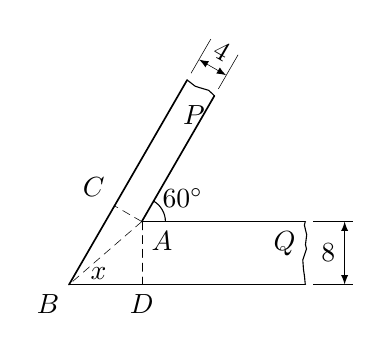
\begin{tikzpicture}[>=latex,scale=1.0]
  \tkzDefPoints{0/0/B,3/0/E,3/0.8/Q}
  \tkzDefPoint(60:3){F}
  \tkzDefShiftPoint[F](-30:0.4){P}
  \tkzDefPointsBy[translation=from E to Q](B){B1}
  \tkzDefPointsBy[translation=from F to P](B){B2}
  \tkzInterLL(B1,Q)(B2,P)\tkzGetPoint{A}
  \tkzDefPointsBy[projection=onto B--E](A){D}
  \tkzDefPointsBy[projection=onto B--F](A){C}
  \tkzDrawSegments[semithick](B,E B,F Q,A P,A)
  \tkzDrawSegments[densely dashed](A,C A,D A,B)
  \tkzLabelPoints[below left](B,P,Q)
  \tkzLabelPoints[below right](A)
  \tkzLabelPoints(D)
  \tkzLabelPoints[above left](C)
  \tkzLabelAngle[pos=0.4](D,B,A){$x$}
  \tkzMarkAngle[size=0.3](Q,A,P)
  \tkzLabelAngle[pos=0.6](Q,A,P){\ang{60}}
  \draw[decorate,decoration={random steps,segment length=3pt,amplitude=1pt}](E)--(Q);
  \draw[decorate,decoration={random steps,segment length=3pt,amplitude=1pt}](F)--(P);
  \draw[very thin] (3.1,0)--(3.6,0)(3.1,0.8)--(3.6,0.8);
  \draw[very thin] ([shift=(60:0.1)]F)--++(60:0.5)([shift=(60:0.1)]P)--++(60:0.5);
  \draw[very thin,<->](3.5,0)--(3.5,0.8)node[midway,left]{8};
  \draw[very thin,<->]([shift=(60:0.3)]F)--([shift=(60:0.3)]P)node[midway,above,sloped]{4};
\end{tikzpicture}
\end{document}